\section{本章小结}
\label{sec:moo-summary}

本章从“两个目标各有所长的方案谁更好”出发。结论是，不依赖偏好的比较只有支配关系，由它得到的是一组互不支配的方案，而不是一个方案。目标冲突不会因为单目标算法更强而消失，强的算法只能更快地解出某一个偏好下的问题。

支配关系是第一层判断，它不受单位影响。权重、距离和归一化都依赖尺度，使用时要写明单位与参考范围。

偏好由三种标量化表达。加权和相当于定价，权重全正的全局解是Pareto最优的，凸问题中非负权重足以选中每个弱Pareto最优点，但在非凸前沿上会遗漏非支撑点。阈值约束相当于定预算，加权Chebyshev相当于要求各项接近某个水平，二者不需要凸性就能选中每个Pareto点，但可能返回并列的弱Pareto最优解，需要第二阶段的择优。

局部信息给出一阶判别。Pareto驻定说明不存在严格共同下降的方向，这是局部弱Pareto最优的必要条件，有约束时要在约束资格下配合乘子；要由它推出全局结论，还需要凸性，权重全正时才能得到Pareto最优。多梯度下降从梯度凸包的最小范数元得到共同下降方向，配合共同步长使每个目标都下降，一次运行收敛到一个驻定点。

要得到一组候选，可以扫描偏好参数，用热启动降低代价，按空缺补点，并用非支配存档保存结果；也可以用NSGA-II这样的群体搜索，以分层和拥挤距离代替单目标的排序。两者都要在固定的目标尺度下，用约束违反、残差、超体积、间距以及到参考前沿的距离来检查。

图~\ref{fig:moo-summary}汇总了四种结果之间的关系。加权最优、Pareto驻定、全局Pareto最优和有限候选集的覆盖是四种不同的结论，从一种到另一种都需要说明所依赖的条件。

\begin{BookInlineFigure}
  \centering
  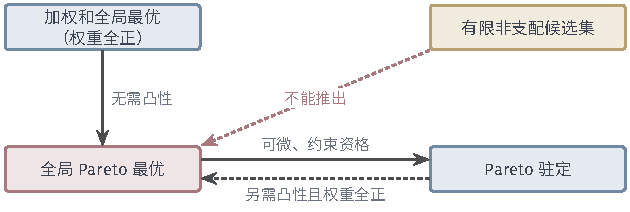
\includegraphics[width=106.7mm]{figures/05-optimization/07-multiple-criteria-and-nested-optimization/tikz/moo-summary/figure.pdf}
  \caption{四种结果的关系。实线箭头在标注的条件下成立，虚线箭头需要额外的条件，红色虚线表示有限候选集互不支配不能推出全局Pareto最优。}
  \label{fig:moo-summary}
\end{BookInlineFigure}
